% This file was created with tikzplotlib v0.10.1.
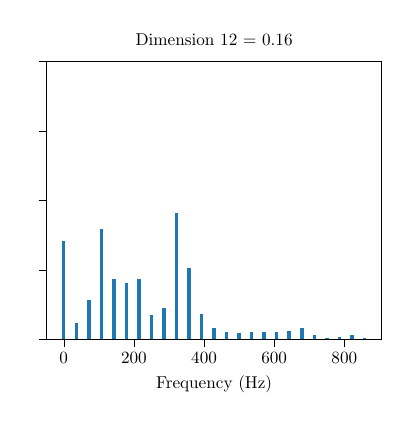
\begin{tikzpicture}[scale=0.62]

\definecolor{darkgray176}{RGB}{176,176,176}
\definecolor{steelblue31119180}{RGB}{31,119,180}

\begin{axis}[
yticklabel={\empty},
tick align=outside,
tick pos=left,
x grid style={darkgray176},
xlabel={Frequency (Hz)},
xmin=-48.3571428571429, xmax=905.5,
xtick style={color=black},
y grid style={darkgray176},
% ylabel={Magnitude},
ymin=0, ymax=4,
title={Dimension 12 = 0.16},
ytick style={color=black}
]
\draw[draw=none,fill=steelblue31119180] (axis cs:-5,0) rectangle (axis cs:5,1.41595725063235);
\draw[draw=none,fill=steelblue31119180] (axis cs:30.7142857142857,0) rectangle (axis cs:40.7142857142857,0.23622781975444);
\draw[draw=none,fill=steelblue31119180] (axis cs:66.4285714285714,0) rectangle (axis cs:76.4285714285714,0.573161569006036);
\draw[draw=none,fill=steelblue31119180] (axis cs:102.142857142857,0) rectangle (axis cs:112.142857142857,1.58223645935967);
\draw[draw=none,fill=steelblue31119180] (axis cs:137.857142857143,0) rectangle (axis cs:147.857142857143,0.875977028634564);
\draw[draw=none,fill=steelblue31119180] (axis cs:173.571428571429,0) rectangle (axis cs:183.571428571429,0.815332302009045);
\draw[draw=none,fill=steelblue31119180] (axis cs:209.285714285714,0) rectangle (axis cs:219.285714285714,0.864334399396921);
\draw[draw=none,fill=steelblue31119180] (axis cs:245,0) rectangle (axis cs:255,0.349835513693747);
\draw[draw=none,fill=steelblue31119180] (axis cs:280.714285714286,0) rectangle (axis cs:290.714285714286,0.448775700460644);
\draw[draw=none,fill=steelblue31119180] (axis cs:316.428571428571,0) rectangle (axis cs:326.428571428571,1.81389758244189);
\draw[draw=none,fill=steelblue31119180] (axis cs:352.142857142857,0) rectangle (axis cs:362.142857142857,1.02524061550871);
\draw[draw=none,fill=steelblue31119180] (axis cs:387.857142857143,0) rectangle (axis cs:397.857142857143,0.358886421061486);
\draw[draw=none,fill=steelblue31119180] (axis cs:423.571428571429,0) rectangle (axis cs:433.571428571429,0.162085935693807);
\draw[draw=none,fill=steelblue31119180] (axis cs:459.285714285714,0) rectangle (axis cs:469.285714285714,0.10709757098892);
\draw[draw=none,fill=steelblue31119180] (axis cs:495,0) rectangle (axis cs:505,0.0909466928673103);
\draw[draw=none,fill=steelblue31119180] (axis cs:530.714285714286,0) rectangle (axis cs:540.714285714286,0.103740986056779);
\draw[draw=none,fill=steelblue31119180] (axis cs:566.428571428571,0) rectangle (axis cs:576.428571428571,0.113372407747774);
\draw[draw=none,fill=steelblue31119180] (axis cs:602.142857142857,0) rectangle (axis cs:612.142857142857,0.106204828941314);
\draw[draw=none,fill=steelblue31119180] (axis cs:637.857142857143,0) rectangle (axis cs:647.857142857143,0.119934885317498);
\draw[draw=none,fill=steelblue31119180] (axis cs:673.571428571429,0) rectangle (axis cs:683.571428571429,0.168605714057006);
\draw[draw=none,fill=steelblue31119180] (axis cs:709.285714285714,0) rectangle (axis cs:719.285714285714,0.0627754199635873);
\draw[draw=none,fill=steelblue31119180] (axis cs:745,0) rectangle (axis cs:755,0.02344118249165);
\draw[draw=none,fill=steelblue31119180] (axis cs:780.714285714286,0) rectangle (axis cs:790.714285714286,0.0377101453321494);
\draw[draw=none,fill=steelblue31119180] (axis cs:816.428571428571,0) rectangle (axis cs:826.428571428571,0.0568180684048655);
\draw[draw=none,fill=steelblue31119180] (axis cs:852.142857142857,0) rectangle (axis cs:862.142857142857,0.0271239648715643);
\end{axis}

\end{tikzpicture}
